
\documentclass{article}

\usepackage[margin=4cm]{geometry}
\usepackage{polyglossia}
	\setmainlanguage{english}
\usepackage{amsmath}
\usepackage{amssymb}
\usepackage{siunitx}
\usepackage{float}
\usepackage{booktabs}
\usepackage{subcaption}
\usepackage{graphicx}
\usepackage{xcolor}
\usepackage{listings}
    \lstset{language=Python,
	basicstyle=\footnotesize\ttfamily,
	breaklines=true,
	framextopmargin=50pt,
	frame=bottomline,
	backgroundcolor=\color{white!85!black},
	commentstyle=\color{blue},
	keywordstyle=\color{red},
	stringstyle=\color{orange!80!black}}
\usepackage{tikz}

\title{Computational Physics - Exercise 8}
\author{Maurice Donner \and Lukas Häffner}

\begin{document}

\maketitle
\newpage

\section{Fixed Points of the Lorenz dynamical System}

The Lorenz attractor problem is given by the following coupled set of 
differential equations
\begin{align}
    \dot x &= - \sigma (x - y ) \\
    \dot y &= rx - y - xz \\
    \dot z &= xy - bz
    \label{Lorenz}
\end{align}
The fixed points for this problem are \( \lambda_1 = (0,0,0) \) for all \( r \)
and \( \lambda_{2,3} = (\pm a_0, \pm a_0, r-1 )\) with \( a_0 = 
    \sqrt{b(r-1)}\) for \( r > 1 \).\\
In this exercise we want to examine the stability of \( \lambda_{2,3} \) by the
Jacobian taken at the fixed points, and then looking for its eigenvalues by means
of finding the zero points of the following characteristic polynomial:
\begin{align}
    P(\lambda) = \lambda^3 + (1+b+\sigma)\lambda^2 +b(\sigma+r)\lambda
    + 2 \sigma b (r-1)
\end{align}
We first plot $P(\lambda)$ as a function of \( \lambda \). For that we use
\( \sigma = 10, b = 8/3 \):
\begin{figure}[H]
    \centering
    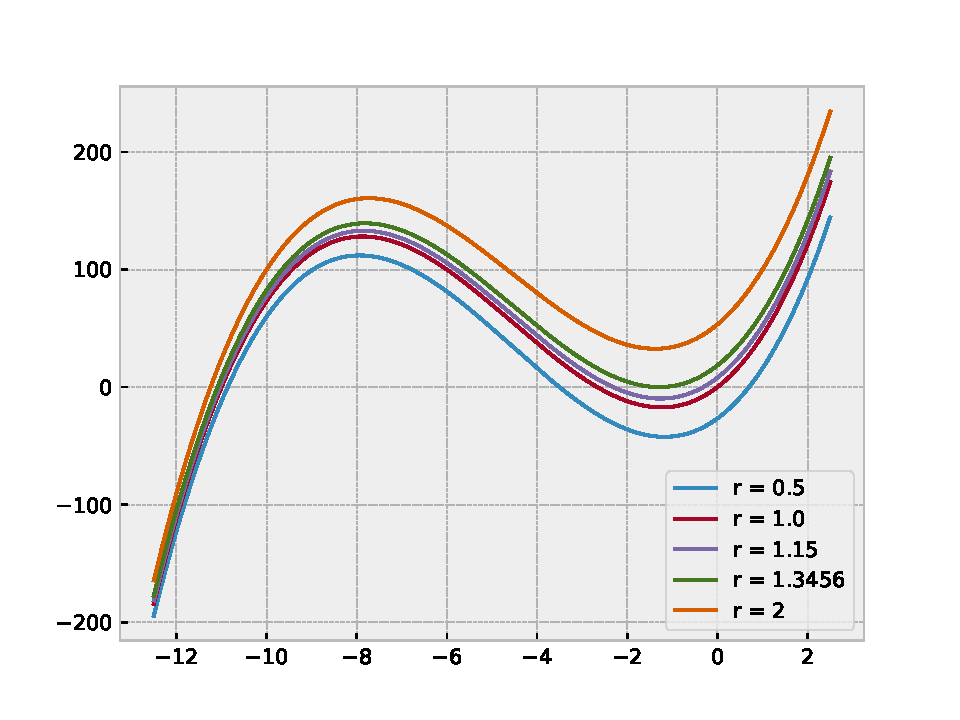
\includegraphics[width=9cm]{polynomial.pdf} 
    \caption{Characteristic Polynomial of the Lorenz attractor} 
\end{figure}
To check if the points are stable, one has to examine the eigenvalues of the
Jacobimatrix at the stationary point. If an eigenvalue has a positive real part,
then the point is unstable. If all realparts are negative the point is stable.
That means:
\begin{table}[H]
    \centering
    \begin{tabular}{ll}
    For $ r < 1 $ & All Solutions unstable, because there is always at least
    one \( \lambda > 0 \) \\ 
    For $ 1 < r < 1.3456 $ & all \( \lambda < 0 \) and the Solution is stable \\
    For $ r > 1.3456 $ & two of the three roots vanish, and the remaining root
    is $ < 0 $, \\ & so in theory, those solutions are stable too.
    \end{tabular}
\end{table}
Note, that this is only correct for the characteristic Polynomial. Later we will
see that the Fix Point \( (0,0,0) \) at \( r < 1 \) is indeed stable, since
the Jacobian has a different shape, and hence, there is a different polynomial.
In the "smaller" case the only fixpoint is $x=y=z=0$ and all eigenvalues of
the resulting Jacobimatrix are negative (shown in
lecture at 12.6). As a result, the simulations for r < 0 reach the
stable point of $x=y=z=0$ in Figure (\ref{2-1}). \\[.5cm]

Next we determine the (complex) roots for different values of r:
\begin{figure}[H]
    \centering
    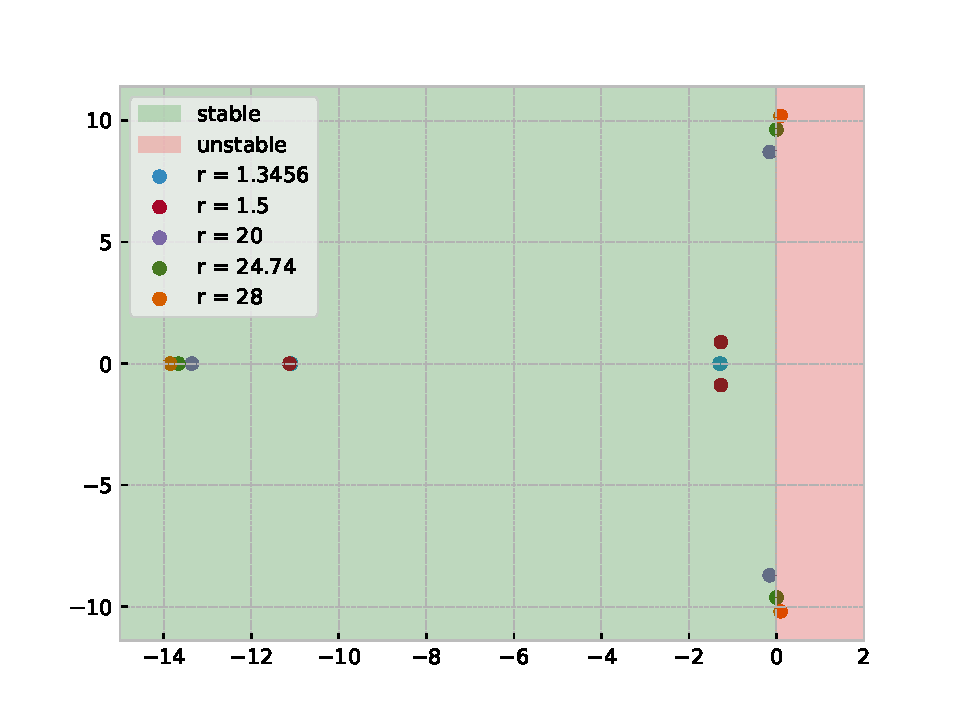
\includegraphics[width=9cm]{Figure1-2.pdf} 
    \caption{(Complex) roots of the Characteristic Polynomial} 
\end{figure}
For \( 1 < r < r_\text{crit,1} = 1.3456 \), all Fixpoints are \( < 0 \) and real,
and are hence stable.\\
For \(  r_\text{crit,1} < r < r_\text{crit,2} = 24.74\), the real parts of the
fixed points are still \( < 0 \) and the Fixpoints (including the complex
conjugate ones) are hence stable. \\
For \( r > r_\text{crit,2} \), the real part of the complex conjugate roots
becomes \( > 0 \). The Fixed points are hence unstable. \\

\section{The Lorenz attractor}
We solve the Lorenz equations numerically with \texttt{rk4}, for the values
\( r = 0.5, 1.15, 1.3456, 24 \ \text{and} \ 28 \).
For that we use the previously integrated Runge-Kutta-4 algorithm
(see Exercise 2). All we need to do is to integrate the coupled Lorenz equations:
\begin{lstlisting}
def f(y0,x0): # y0 array that consists of [x,y,z]
    deriv = np.array([
    - sig*(y0[0] - y0[1]),
    r*y0[0] - y0[1] - y0[0]*y0[2],
    y0[0]*y0[1] - b*y0[2]])

    return deriv
\end{lstlisting}
Using \texttt{rk4}, we plot the trajectories for all \( r \) each with Starting
point \( C_+ \ \text{and} \ C_- \):
\begin{figure}[H]
    \centering
    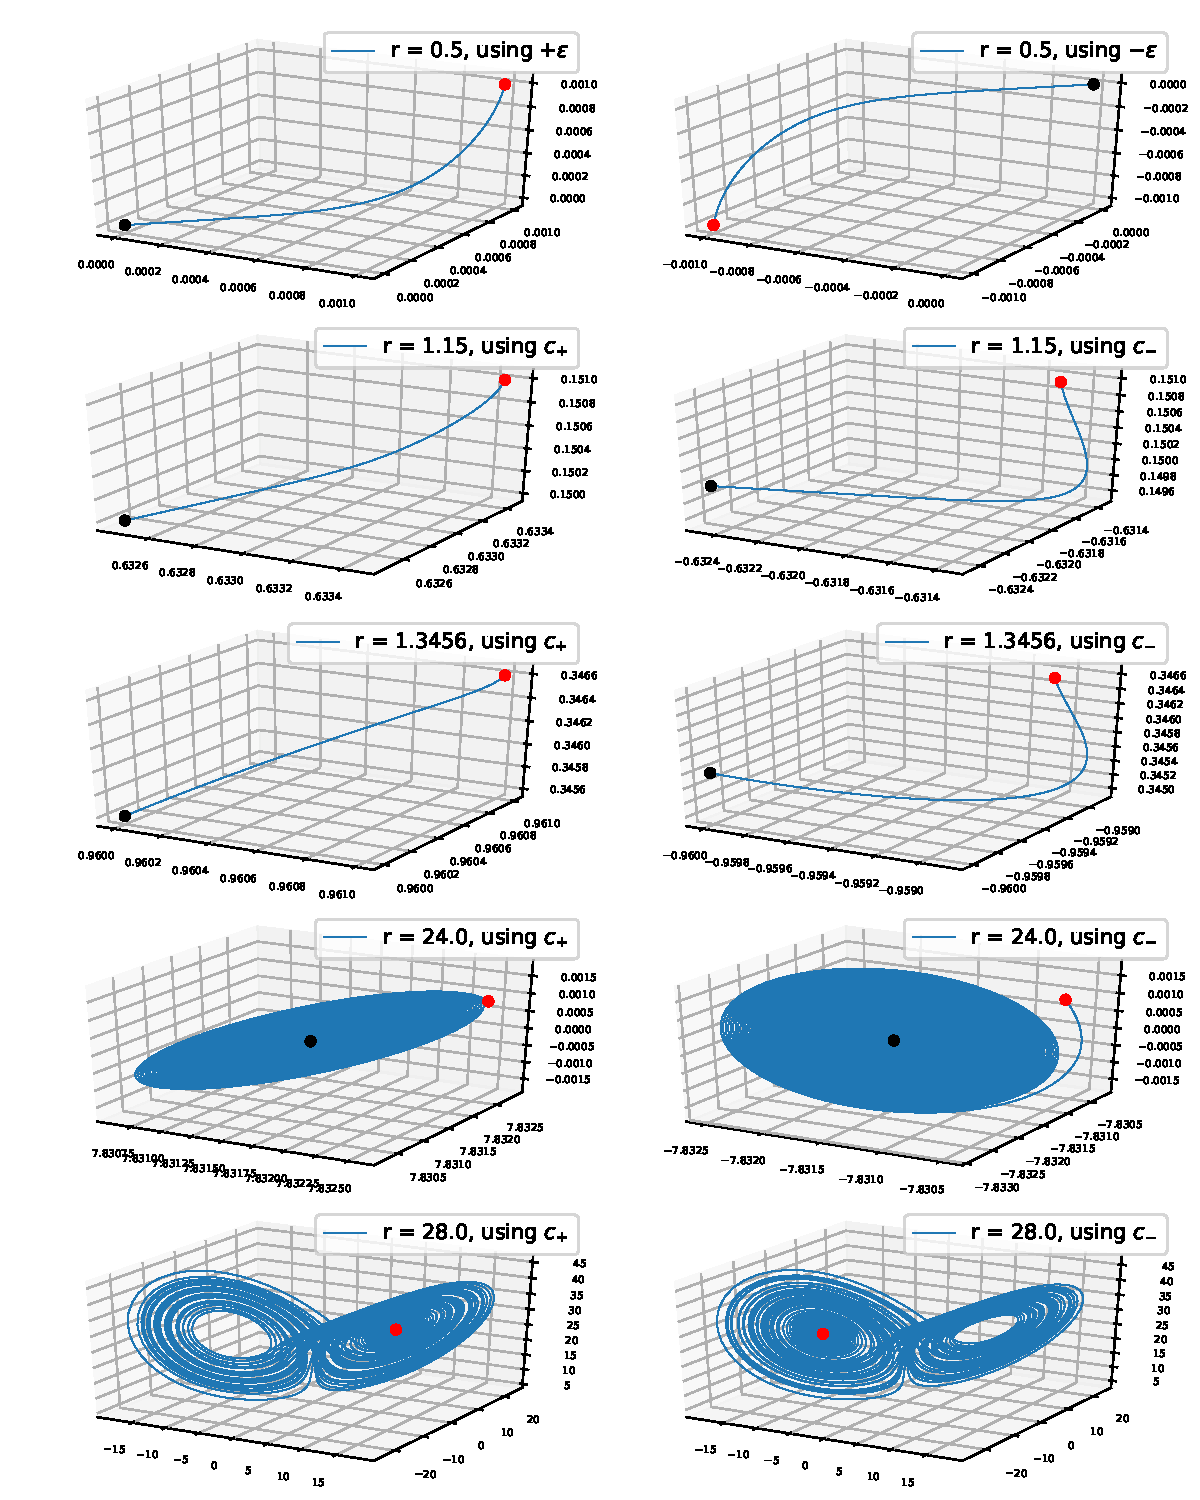
\includegraphics[width=\textwidth]{Figure2-1.pdf} 
    \caption{Determining Fixed points of the Lorenz dynamical System
    (the red dot describes the starting point, the black dot the fix point)} 
    \label{2-1}
\end{figure}
As discussed before, the fixed points for $r < 1$ are stable. The same app The
same applies to all other points until we hit the value \( r_\text{crit,2}
    \approx 24.74\). Here, there is an oscillation around the fixed point that
goes on for a while. For large enough \( t \), a second "disk" emerges, and the
oscillation changes back and forth between the two.
\end{document}

